
\section{Lake Results}

The compiled dataset with n=112 observations with some missing values.


Microcystin concentration displayed a slight curve when plotted against time peaking in the month of August. The average were low in June and October()

In our toxin analysis, we did not detect any cylindrospermonsin in our survey. We had one instance of anatoxin-a detected at Brighton lake in August 2017. From our QPCR analysis, we did not find any genes responsible for producing cylindrospermonsin (\emph{cyrA}), saxitoxin (\emph{sxtA}).  We found microcystin concentrations vary for each lake and through time. MC-RR, MC-LR and MC-LA were the most detected congeners in our survey. MC-RR was found with the highest concentrations 8.55 $\mu$g/L at Brighton Lake. We found varying amounts of \emph{mcyE} gene copies in each lake. Majority of our samples were below the EPA guidance level. From our sampled lake sites, Belleville, Brighton, Ford, Hudson, and Wixom Lake had instances of microcystin concentrations that exceeded the EPA guidance level of 4 $\mu$g/L (see figure \ref{microcystin}).

Mostly all of our sampled lakes were mostly alkaline conditions averaging around 8.53$\pm$0.37 pH ranging from 7.44 to 9.94. Dissolved oxygen averaged around 12.98$\pm$20.8 mg/L of \ch{O2}.

\section{\emph{A Priori} Hypothesis Test}

There were a slight positive trend with developed land-use plotted with log10(MC) concentration ,however the relationship is not significant  ($\beta=0.59$, $F_{{1,27}}=1.75$ , $p=0.20$). There was also no significant relationship between log10\emph{mcyE} gene copies and developed land use ($\beta=0.62$, $F_{{1,27}}=1.08$ , $p=0.30$), or with log10(\emph{16S rRNA}) gene copies ($\beta=0.48$, $F_{{1,25}}=1.75$ , $p=0.27$).
The amount  of zebra mussels did not significantly affect any of our response variables.
Forest land use had a significant negative relationship with \emph{16s rRNA} gene copies ($\beta=-1.42$, $F_{{1,25}}=7.08$, $p=0.013$). Albiet, forest land use did not have a significant effect on microcystin concentrations ($\beta=-0.34$, $F_{{1,26}}=0.32$, $p=0.57$).
The 16S rRNA gene copies has a signification positive relationship with microcystin concentrations.

Observing our correlation matrix (see \ref{matrix}), we can see some correlation between some of our variables. Land-use with nutrient concentrations. Agriculture had a positive effect on nitrate+nitrite,



\section{Feature Selection}

From our best subset analysis with the largest subset size of 4 (nvmax=4), we chose orthophosphate, total phosphate, turbidity,  and mcyE gene as our full model as its frequently chosen and persistent in each iteration (see figure \ref{subset}).

Total phosphate was not a signifigant predictor ($\beta=0.49$, $F_{{1,27}}=0.45$ $p=0.50$).
Microcystin concentration was signifigantly correlated with turbidity {$\beta=0.29$, $F_{{1,107}}=6.88$ $p=0.01$}

For predictive model for 16S rRNA gene copies, Chloraphyll, agriculture were chosen frequently in the subset analysis \ref{subset2}.

Total phosphorus did not show to have any signifigant relationship with any of our response variable.

\section{Discussions}






From , we wanted to deduce the idea of disturbance from developed land is associated with HABs. Disturbances of flora contributes to lower nutrient retention and hydrological impacts that can cause more blooms \cite{anderson_harmful_2002, codd_cyanobacterial_2000, fraterrigo_influence_2008}. From our data, we did not see a significant relationship between developed land use and any of our nutrient analysis.
Microcystin could increase as developed is more prevalent in the lake's watershed.

Other studies have found this relationship signifigantly positive.
One study on Lake Tai in China seeked to find correlation with fecal bacteria as a surrogate for urbanization and microcystin concentrations \cite{wilhelm_relationships_2011}.
They examined fecal bacteria asscociated with human population as a predictor. They did not find a signifigant correlation between human fecal bacteria and microcystin concentration or algal biomass \cite{wilhelm_relationships_2011}.
A statistical analysis study  on the EPA National Lake Assessment results found microcystin concentrations correlated to percentage of developed land use in the lakes watershed \cite{beaver_land_2014}. However in our data, we do not see a significant relationship. With each lake's watersheds characteristics,

A study in South Korea found 3-week lagged water temperature,dissolved oxygen and pH with to correlate with each other in their models \cite{ahn_evaluation_2011}.
We did not find

Growing cyanobacteria measurements taken at the same time . Their is an assumption being made.

Total nitrogen was found to explain the variance of microcystin concentrations \cite{taranu_predicting_2017}.

Man-made lakes are found to be twice as higher concentrations in cylindrospermonsin \cite{loftin_cyanotoxins_2016}.





Low-nutrient lakes can still exhibit blooms.
Cyanobacteria are versatile as they can acquire nutrients under extreme conditions. They can utilize a process called quorom sensing which they coordinate with each other by using a signaling hormone acylated homoserine lactones \cite{van_mooy_quorum_2012}. This creates a network of cells which work together as a unit, often as seen as a layer of green goo floating on top of water. This can complicate our model as this is not accounted for.

QPCR results as a response variable comes with complication as this does not distinguish alive or dead cyanobacteria.


Biological properties are not necessarily linear. One thing to consider here is the sampling frequency. We sampled once a month for four months, which gives four sampling results for each lake. This may not explain everything about each lake.

Failure to address ecological factors also can fail models. Previous studies in inland Michigan lakes are finding New Zealand Mudsnails to have an impact on finding blooms \cite{vanderploeg_zebra_2001}.


Water sampling for nutrient is difficult. Time series data, nutrient dynamic. Continuous measurements  water data would be best, but for a large survey its almost impractical. Other organisms compete with these common nutrients. Aquatic macrophytes largely acquire dissolved phosphorus. Nutrients acting as a stimulus could be a function similar to the shape of a Michaelis-Menton curve. Time between sampling the lake at the peak of the bloom and the flush of nutrient inputs can be lagged, and most likely different depending on each lakes morphology.

Bioavailability of phosphorus is pH dependent, where most is available between when in alkaline conditions greater \cite{lucas_relationships_1961}.




\begin{table}[!ht]
  \label{variable}
  \caption{List of coded measured variables and transformation}
\centering
\scalebox{0.66}{
\begin{tabular}{lll}
  \hline
Short Name & Variable Name (Units) & Transformation \\
  \hline
OP & Ortho-P (mg-P/L) & log10(OP + 0.003) \\
  NOX & Nitrate/Nitrite (mg-N/L) & log10(NOX + 0.04) \\
  NH3 & Ammonia (mg-N/L) & log10(NH3 + 0.006) \\
  TP & Total phosphorus (mg-P/L) & log10(TP + 0.002) \\
  TKN & Total kjeldahl nitrogen (mg-N/L) & log10(TKN + 0.07) \\
  TNTP & Total nitrogen to total phosphorus ratio & None \\
  X16SRNA & Cyano 16s rRNA gene copies (cp/mL) & log10(X16SRNA + 20) \\
  MCYE & mcyE gene copies (cp/mL) & log10(MCYE + 20) \\
  SUM & Microcysin sum from all 12 MC congeners (ppb) & log10(SUM + 0.03) \\
  wtemp & Water temprature at time of sampling (Celcius) & None \\
  pH & pH & None \\
  do & Dissolved oxygen (mg/L) & log10(do + 0.01) \\
  conduc & Conductance (uS/cm) & log10(conduc + 0.01) \\
  turb & Turbidity (NTU) & log10(turb + 0.01) \\
  chloro & Chloraphyll-a (RFU) & log10(chloro + 0.01) \\
  phyco & Phycocyanin (RFU) & log10(phyco + 0.01) \\
  TN & Total nitrogen (mg-N/L) & log10(TN + 0.116) \\
  Max\_Depth & Maximum depth of lake (meters) & None \\
  Lake\_Area\_sqKm & Lake area (sq Km) & log10(Lake\_Area\_sqKm + 1) \\
  Watershed\_Area\_sqKm & Watershed Area (sq Km) & log10(Watershed\_Area\_sqKm + 1) \\
  Lake Area\_Watershed Ratio & Lake area to watershed area ratio & log10(Lake Area\_Watershed Ratio + 1) \\
  Water & Land-Use percentage in lakes watershed & None \\
  Developed & Land-Use percentage in lakess watershed & None \\
  Barren & Land-Use percentage in lakes watershed & None \\
  Forest & Land-Use percentage in lakes watershed & None \\
  Shrubs & Land-Use percentage in lakes watershed & None \\
  Herbaceous & Land-Use percentage in lakes watershed & None \\
  Agriculture & Land-Use percentage in lakes watershed & None \\
  Wetlands & Land-Use percentage in lakes watershed & None \\
  LogMusselMass & Zebra mussel Mass (grams) & log10(MusselMass + 1) \\
  LogMusselNum & Zebra mussel counts & log10(MusselNum + 1) \\
  precip3 & Average precipitation 3 days before sampling  (mm) & log10(precip3 + 1) \\
  temp3ambient & Average temperature 3 days before sampling (Celcius) & None \\
  precip5 & Average precipitation 5 days before sampling (mm) & log10(precip5 + 1) \\
  temp5ambient & Average temperature 5 days before sampling (Celcius) & None \\
  precip7 & Average precipitation 7 days before sampling (mm) & log10(precip7 + 1) \\
  temp7ambient & Average temperature 7 days before sampling (Celcius) & None \\
  precip30 & Average precipitation 30 days before sampling (mm) & log10(precip30 + 1) \\
  temp30ambinet & Average temperature 30 days before sampling(Celcius) & None \\
  hobotemp & Average Temprature from Hobo pendant one month before sampling (Celcius) & None \\
  hobolight & Average light intensity from Hobo pendant one month before sampling (lux) & log10(hobolight +1) \\
   \hline
\end{tabular}}
\end{table}

\begin{figure}[!ht]
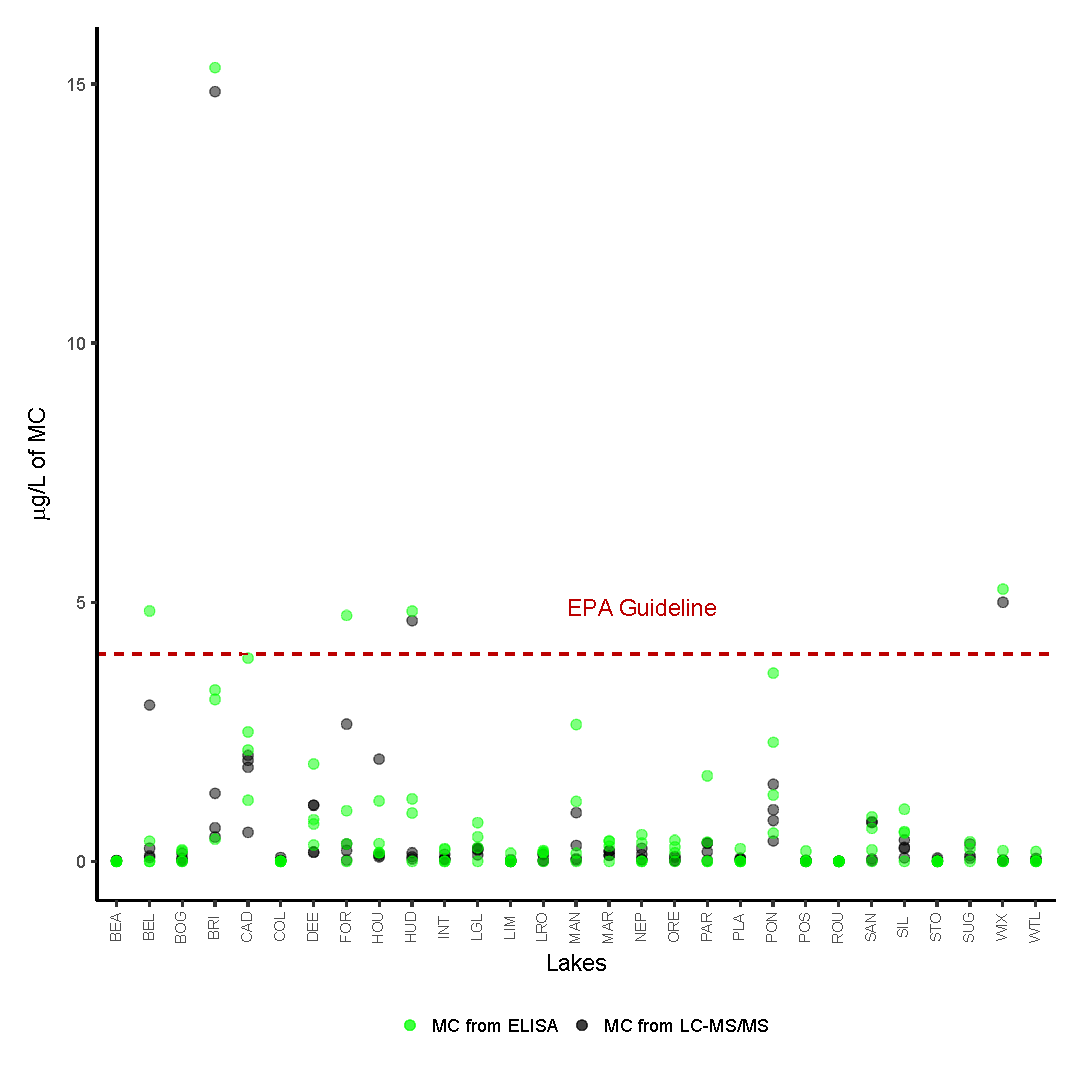
\includegraphics[scale=0.8]{figures/Microcystin}
\caption{Total microcystins by each lake}
\label{microcystin}
Microcystin results from ELISA and LC-MS/MS are plotted by each lake.
\end{figure}

\begin{figure}[!ht]
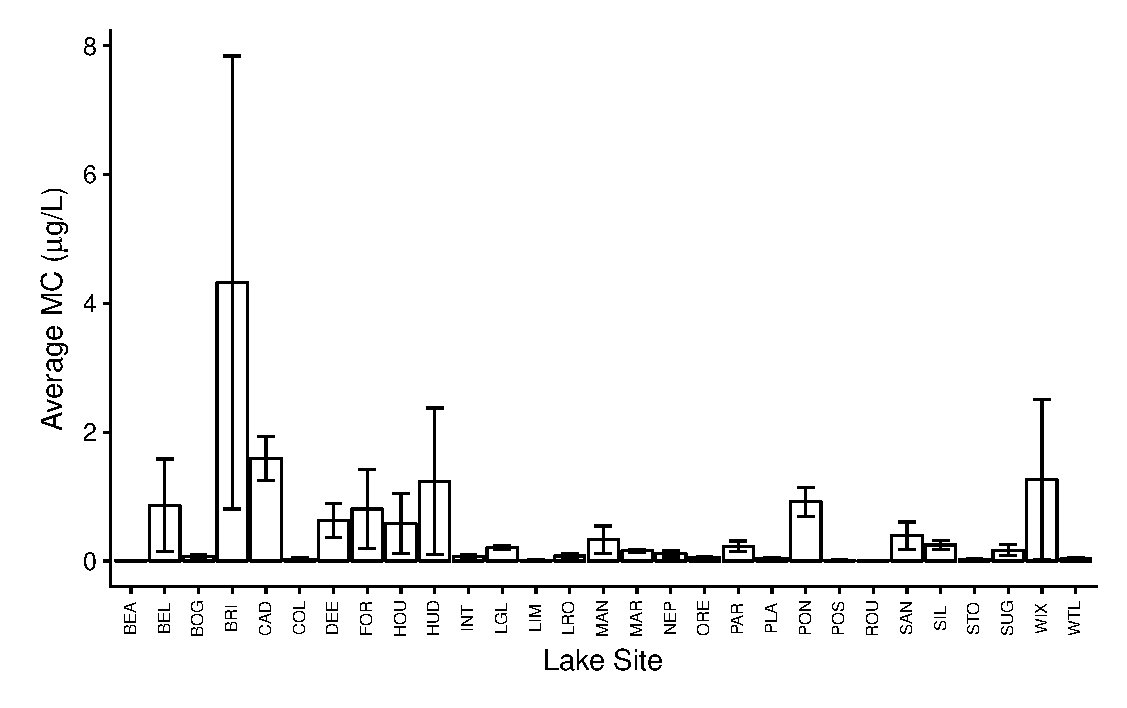
\includegraphics{figures/barmcsum}
\caption{Average total microcystin of each lake measured by LC-MS/MS}
\label{mcbar}
\end{figure}



\begin{figure}[!ht]
  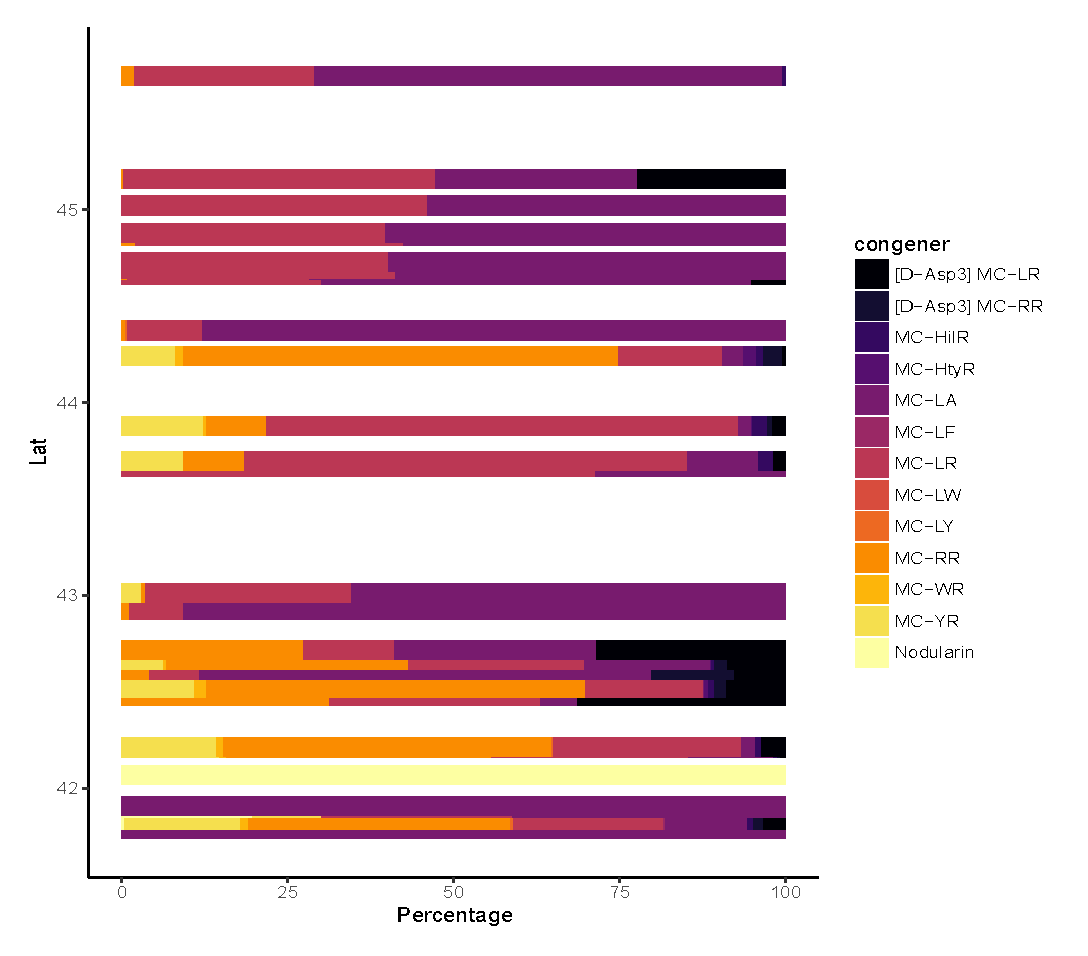
\includegraphics[scale=0.9]{congeners}
    \caption{Proportion of MC congeners plotted by latitude}
  \label{congenerlat}
\end{figure}

\begin{figure}[!ht]
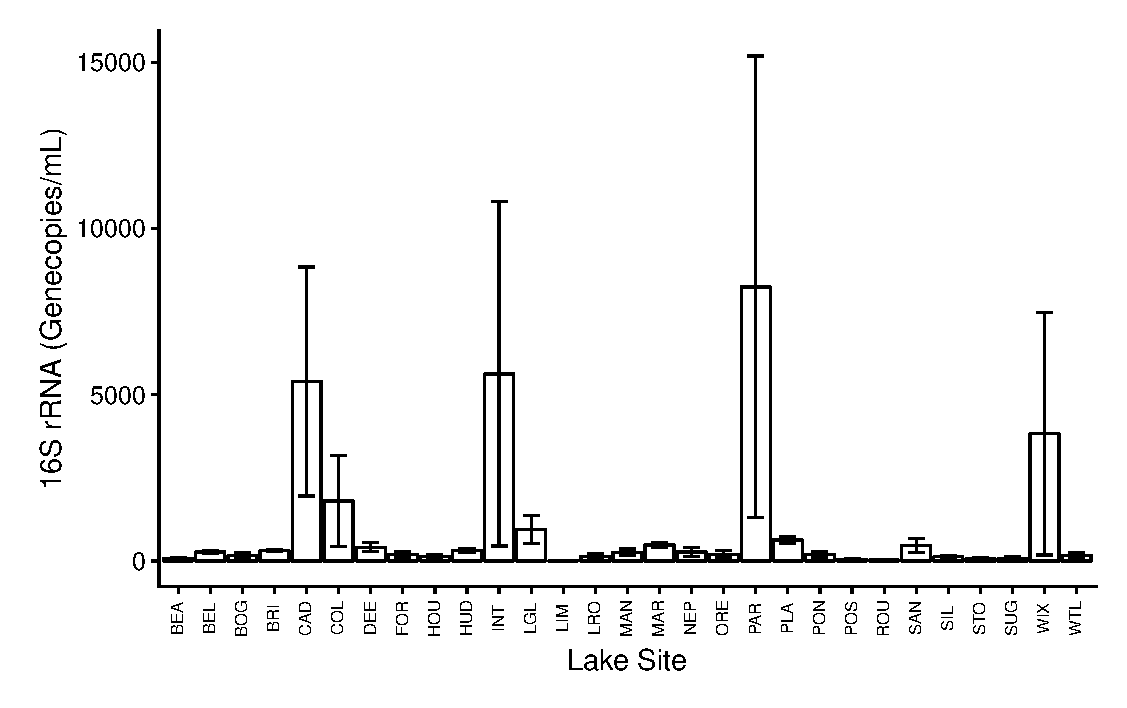
\includegraphics{figures/bar16srna}
\caption{Average 16S rRNA Genecopies/mL of sample by each lake}
\label{box16srna}
\end{figure}

\begin{table}[!ht]
\centering
  \caption{Microcystin congener statistical summary}
  \label{}
\begin{tabular}{@{\extracolsep{5pt}}lccccc}
\\[-1.8ex]\hline
\hline \\[-1.8ex]
Statistic & \multicolumn{1}{c}{N} & \multicolumn{1}{c}{Mean} & \multicolumn{1}{c}{St. Dev.} & \multicolumn{1}{c}{Min} & \multicolumn{1}{c}{Max} \\
\hline \\[-1.8ex]
Nodularin & 114 & 0.0003 & 0.002 & ND & 0.021 \\
{[D-Asp3]}MC-RR & 114 & 0.006 & 0.028 & ND & 0.255 \\
MC-RR & 114 & 0.185 & 0.855 & ND & 8.552 \\
MC-YR & 114 & 0.046 & 0.202 & ND & 1.799 \\
MC-HtyR & 114 & 0.002 & 0.012 & ND & 0.107 \\
MC-LR & 114 & 0.142 & 0.447 & ND & 3.570 \\
{[D-Asp3]}MC-LR & 114 & 0.027 & 0.107 & ND & 0.902 \\
MC-HilR & 114 & 0.004 & 0.019 & ND & 0.150 \\
MC-WR & 114 & 0.005 & 0.029 & ND & 0.302 \\
MC-LA & 114 & 0.088 & 0.196 & ND & 1.729 \\
MC-LY & 114 & 0.0004 & 0.002 & ND & 0.024 \\
MC-LW & 114 & ND & ND & ND & ND \\
MC-LF & 114 & 0.0002 & 0.001 & ND & 0.012 \\
MC Sum from LC MS/MS  & 114 & 0.505 & 1.580 & ND & 14.857 \\
MC from ELISA & 115 & 0.747 & 1.784 & ND & 15.320 \\
\hline \\[-1.8ex]
\multicolumn{6}{r}{Values are expressed as($\mu$g of MC*${L^{-1}}$)} \\
\end{tabular}
\end{table}



\begin{table}[!ht]
  \centering
  \caption{QPCR statistical summary table}
  \label{QPCR}
  \begin{tabular}{@{\extracolsep{5pt}}lccccc}
  \\[-1.8ex]\hline
  \hline \\[-1.8ex]
  Statistic & \multicolumn{1}{c}{N} & \multicolumn{1}{c}{Mean} & \multicolumn{1}{c}{St. Dev.} & \multicolumn{1}{c}{Min} & \multicolumn{1}{c}{Max} \\
  \hline \\[-1.8ex]
  16S rRNA & 112 & 405,761 & 798,946 & ND & 6,765,631 \\
  mcyE & 91 & 8,517 & 49,396 & ND & 467,174 \\
  cyrA & 93 & ND & ND & ND & ND \\
  sxtA & 93 & ND & ND & ND & ND \\
  \hline \\[-1.8ex]
  \multicolumn{6}{r}{* Values are expressed as Gene copies/$\mu$L} \\
  \multicolumn{6}{r}{ND=No Detects} \\
  \end{tabular}
  \end{table}



  \begin{figure}[!ht]
  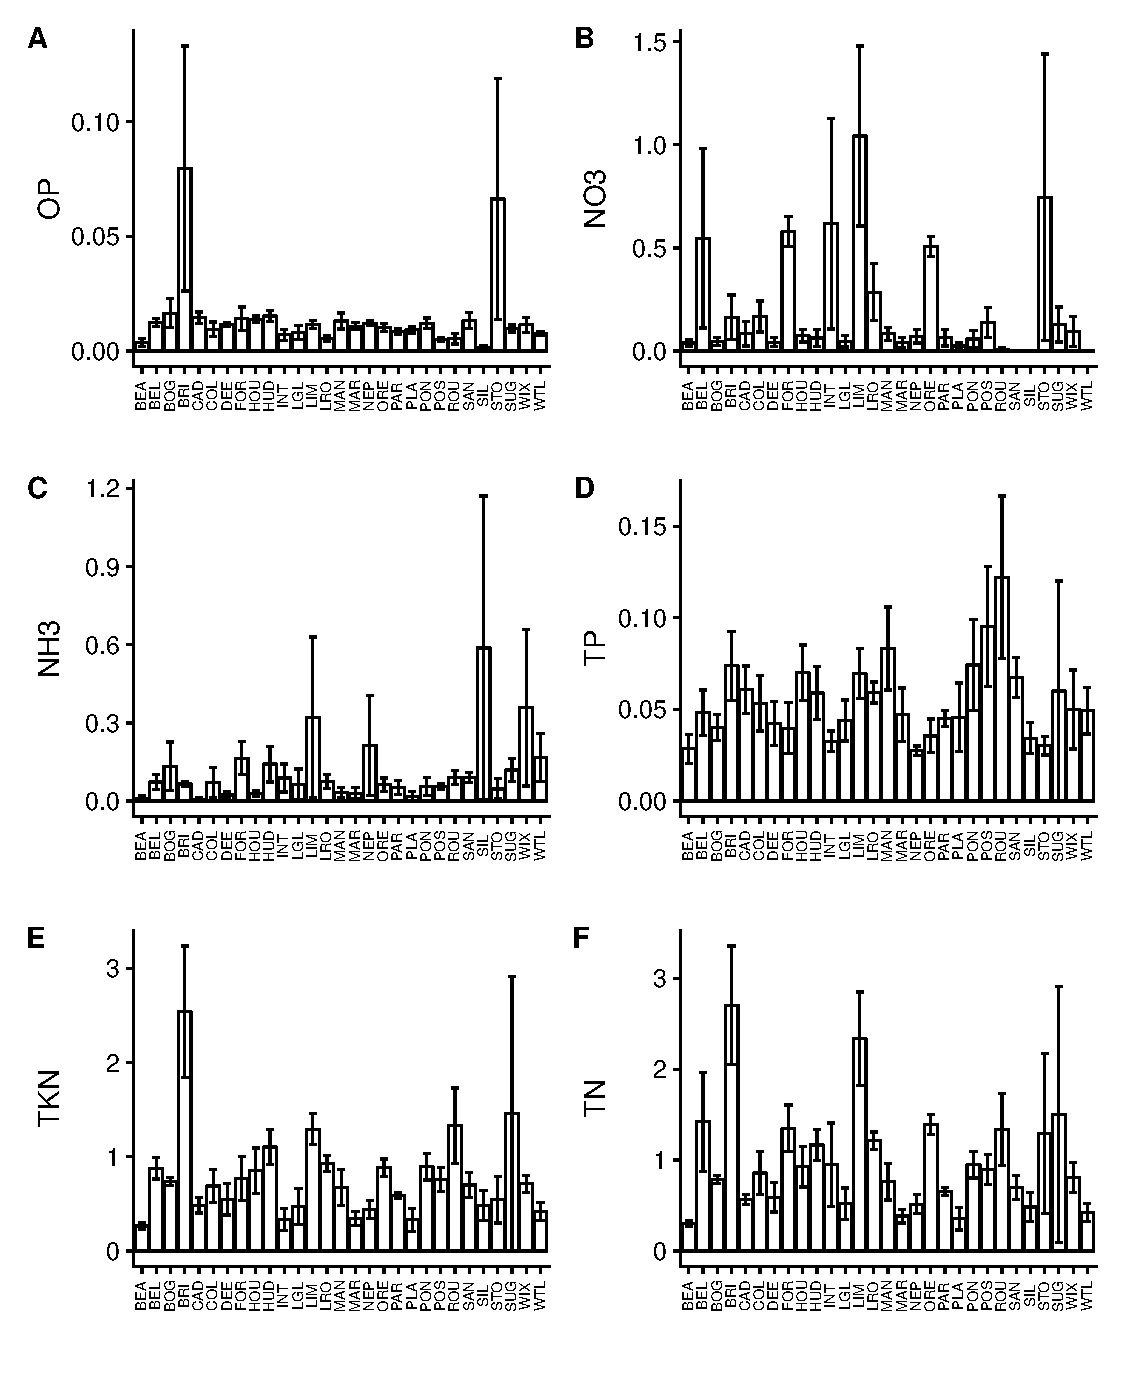
\includegraphics[width=\textwidth, height=15cm]{figures/nutboxplotlake}
  \caption{Nutrients}
  \end{figure}




  \begin{table}[!ht]
    \centering
    \caption{Lake nutrients statistical summary}
    \label{}
  \begin{tabular}{@{\extracolsep{5pt}}lccccc}
  \\[-1.8ex]\hline
  \hline \\[-1.8ex]
  Statistic & \multicolumn{1}{c}{N} & \multicolumn{1}{c}{Mean} & \multicolumn{1}{c}{St. Dev.} & \multicolumn{1}{c}{Min} & \multicolumn{1}{c}{Max} \\
  \hline \\[-1.8ex]
   Orthophosphate (mg P/L) & 114 & 0.015 & 0.030 & 0.000 & 0.237 \\
  Nitrate+Nitrite (mg N/L) & 115 & 0.199 & 0.443 & 0.000 & 2.827 \\
  Ammonia (mg N/L)  & 115 & 0.112 & 0.281 & 0.000 & 2.338 \\
  Total Phosphorus (mg P/L) & 114 & 0.055 & 0.037 & 0.000 & 0.239 \\
  Total Kjeldahl Nitrogen (mg N/L) & 114 & 0.763 & 0.602 & 0.000 & 4.555 \\
  Total Nitrogen & 114 & 1.074 & 0.870 & 0.103 & 4.717 \\
  \hline \\[-1.8ex]
  \end{tabular}
  \end{table}





\begin{figure}[!ht]
  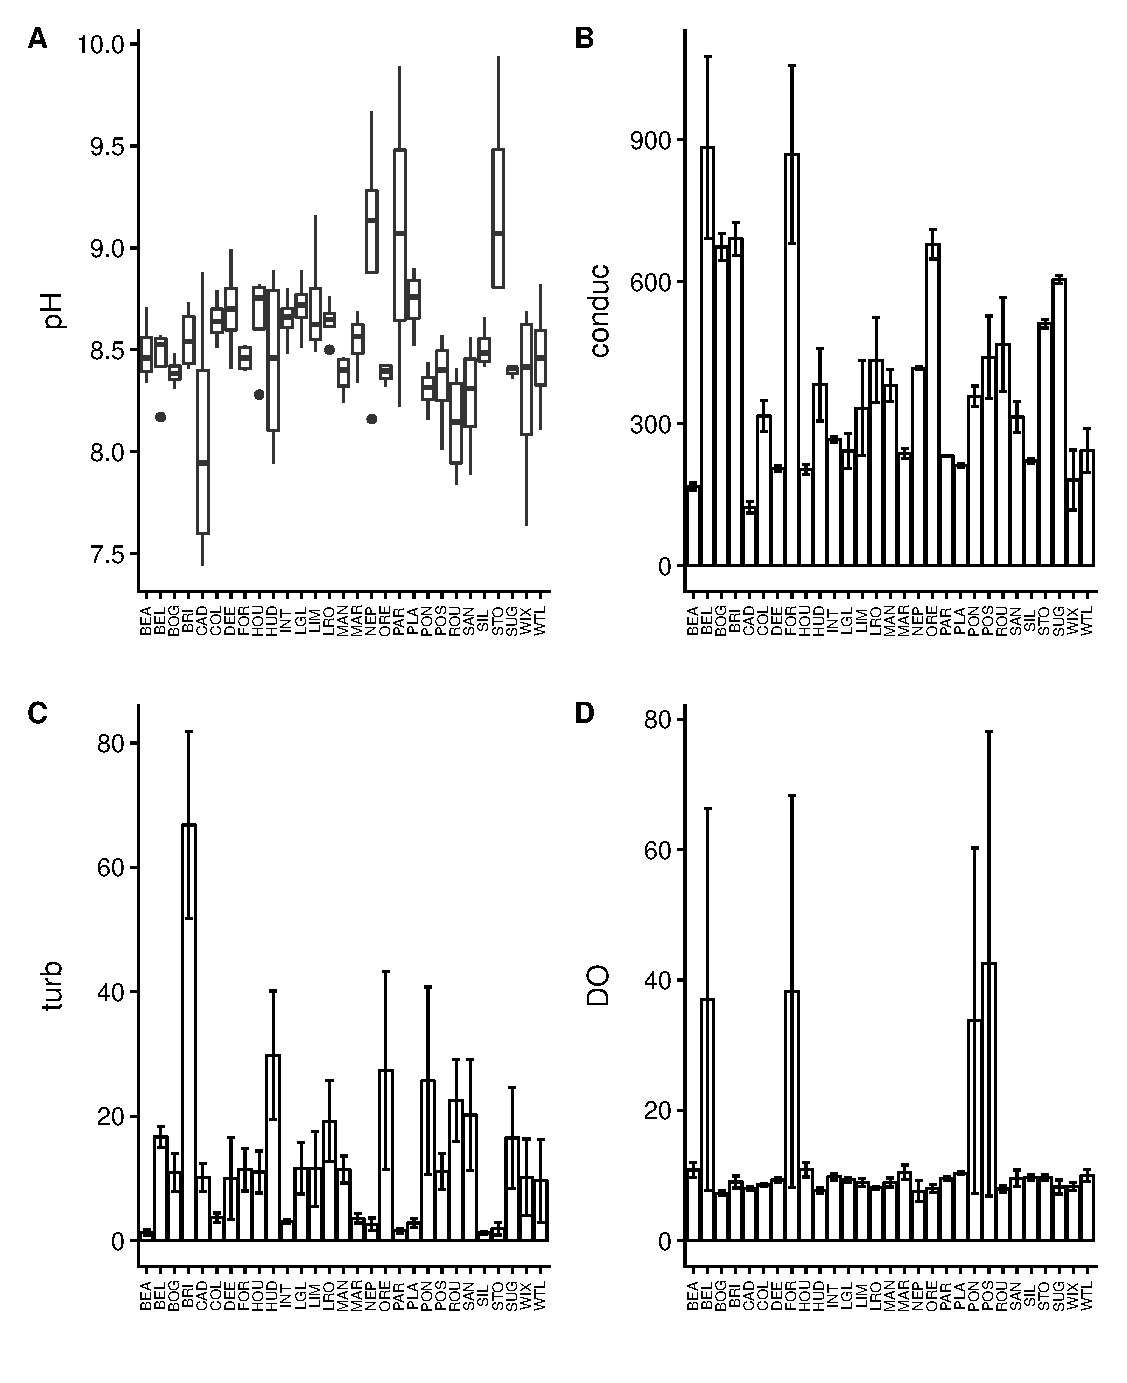
\includegraphics{figures/watboxplotlake.eps}
  \caption{Water chemical parameters}
  (A) Boxplot of pH for all (A).
\end{figure}



\clearpage
\newpage


\begin{figure}[!ht]
  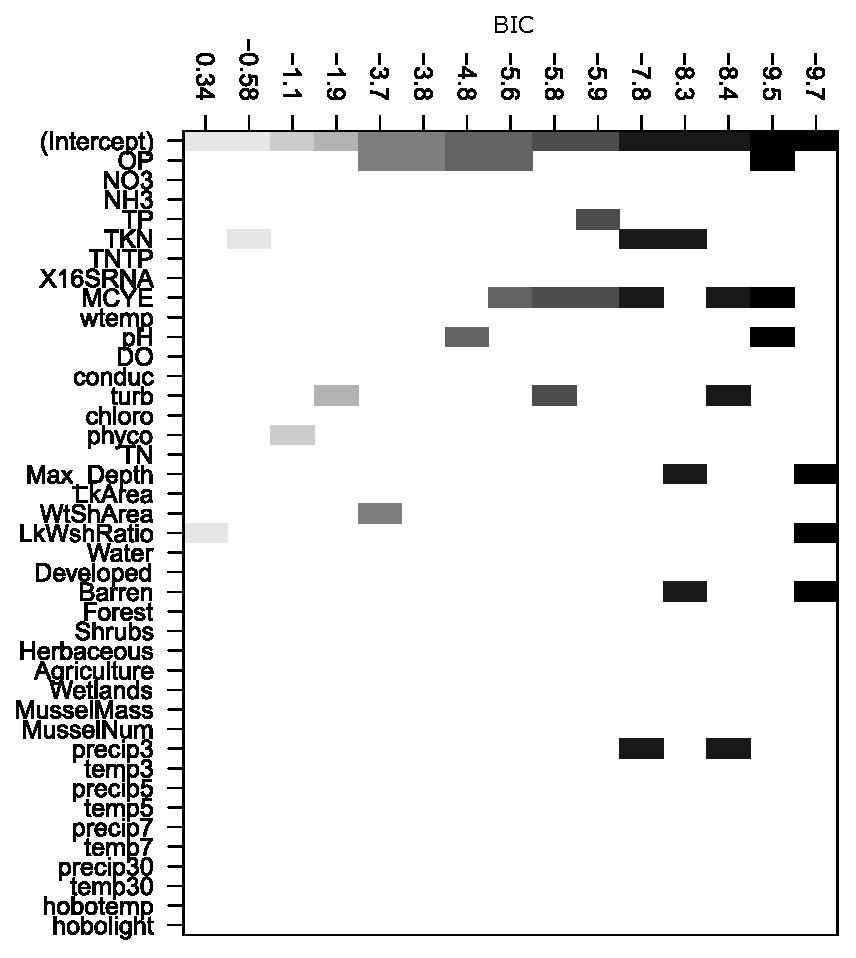
\includegraphics[width=\textwidth]{Subset}
  \caption{Best Subset: MC Sum from LC-MS/MS as response variable}
  \label{subset}
  Each row is a model, if a variable is included in the model it is represented as a shaded rectangle. The BIC is plotted on the y axis where the lowest value is higher up on the axis. The better the model, the lower the BIC, thus the top rows are the better model.
\end{figure}

\begin{figure}[!ht]
  \caption{Correlation Matrix}
  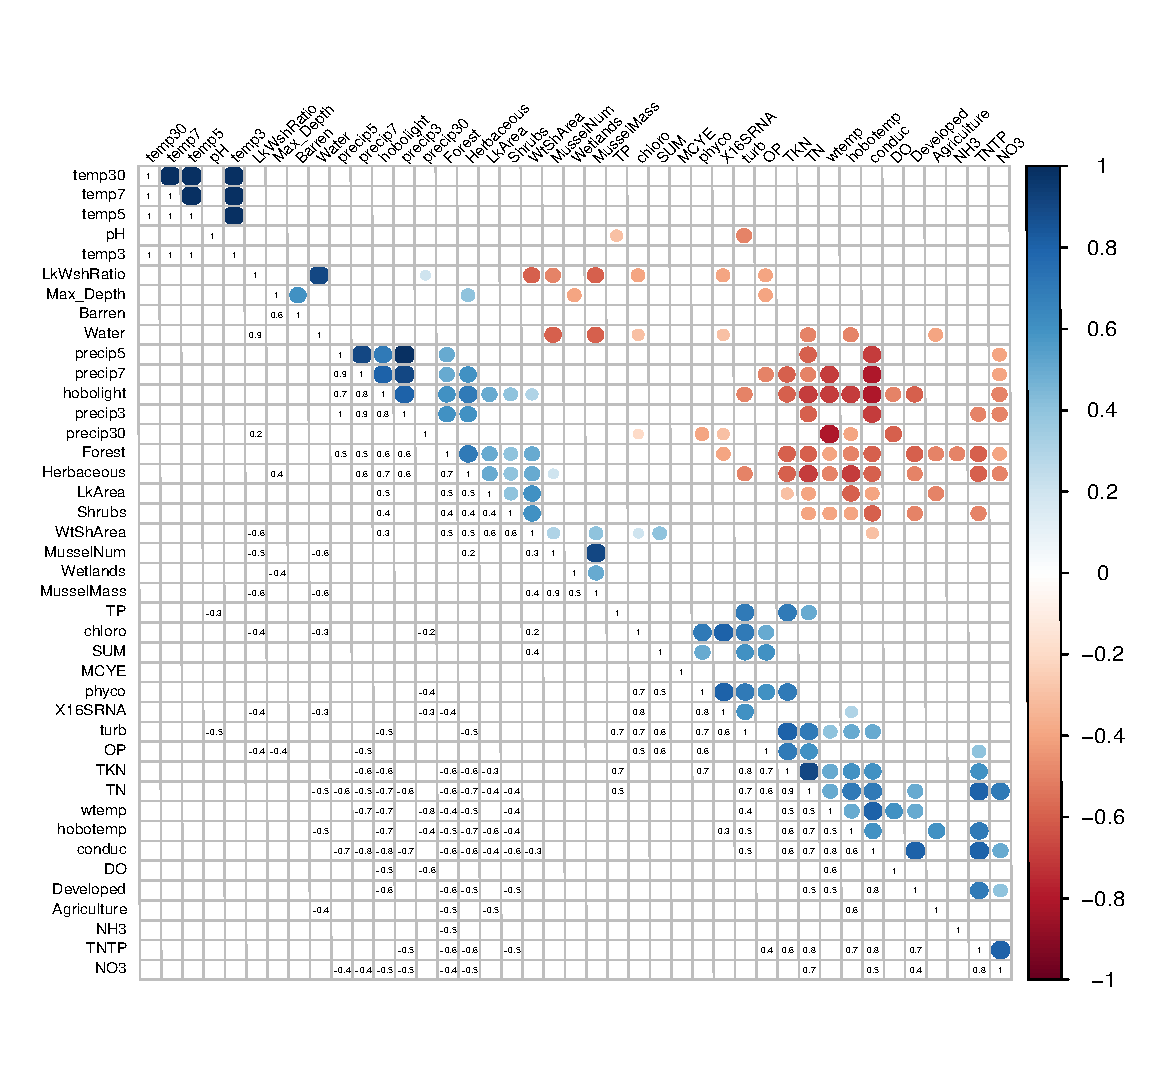
\includegraphics{matrix}
  Positive correlation is represented with solid blue box and negative correlation with scored box.
  \label{matrix}
\end{figure}



\begin{figure}[!ht]
  \includegraphics{Subset2}
  \caption{Best Subset: \emph{16s rRNA} Gene copies as response variable}
  \label{subset2}
\end{figure}
